\subsubsection{Stochastinis gradientinis nusileidimas}
\label{subsubsec:klasifikavimo_tikslumas_stochastinis_gradientinis_nusileidimas}

Stochastinio metodo tikslumas taip pat greitai auga ir pasiekia $97{,}9\ \%$ mokymo duomenims bei $99{,}1\ \%$ validavimo duomenims (žr.~\ref{fig:accuracy_sgd} pav.). Validavimo tikslumas yra aukštesnis nei paketinio metodo atveju.

\begin{figure}[H]
    \centering
    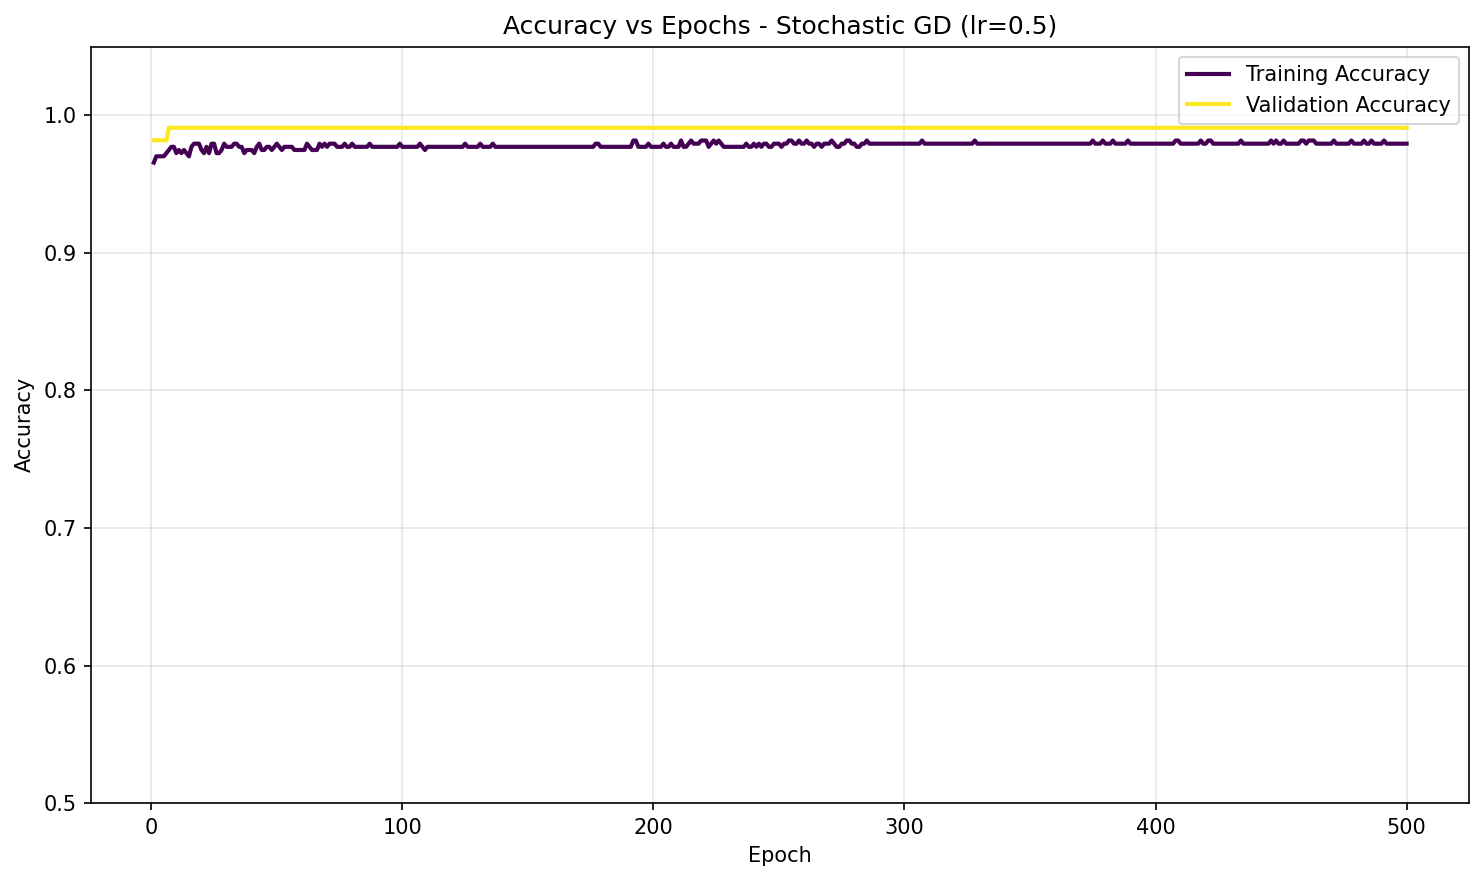
\includegraphics[width=0.85\linewidth]{2Lab/visualizations/accuracy_sgd.png}
    \caption{Klasifikavimo tikslumo priklausomybė nuo epochų (stochastinis GN, $\eta = 0{,}5$)}
    \label{fig:accuracy_sgd}
\end{figure}